\documentclass[12pt,letterpaper]{article}

\usepackage[utf8]{inputenc}
\usepackage[T1]{fontenc}
\usepackage{amsmath}
\usepackage{amsfonts}
\usepackage{amssymb}
\usepackage{amsthm}
\usepackage[left=2cm,right=2cm,top=2cm,bottom=2cm,headheight=22pt]{geometry}
\usepackage{fancyhdr}
\usepackage{setspace}
\usepackage{lastpage}
\usepackage{graphicx}
\usepackage{caption}
\usepackage{subcaption}
\usepackage{paralist}
\usepackage{url}

\theoremstyle{definition}
\newtheorem{question}{Question}
\newtheorem{example}{Example}
\newtheorem{exercise}[question]{Exercise}
\newtheorem*{challenge}{Challenge}
\newtheorem*{theorem}{Theorem}
\newtheorem*{definition}{Definition}

\begin{document}

%Paramètres de mise en forme des paragraphes selon les normes françaises
\setlength{\parskip}{1ex plus 0.5ex minus 0.2ex}
\setlength{\parindent}{0pt}

%Paramètres relatifs aux en-têtes et pieds de page.
\pagestyle{fancy}
\lhead{Theron J Hitchman}
\chead{\Large Reading and Guided Practice \#06}
\rhead{Spring 2016}
\lfoot{\emph{Math and Decision Making}}
\cfoot{}
\rfoot{\emph{\thepage\ of \pageref{LastPage}}}

\section*{Introduction}

In this lesson, you will learn about an \emph{algorithm}, and another theorem due to Euler that
settles the K\"{o}nigsberg bridges problem for any graph.

\section*{Goals}
At the end of this assignment, a student should be able to:
\begin{compactitem}
\item state and use a theorem by Euler about special cycles on graphs,
\item discuss what an algorithm is, and
\item implement an algorithm that finds Eulerian cycles.
\end{compactitem}
A student might also be able to:
\begin{compactitem}
\item Solve a challenge that generalizes the K\"{o}nigsberg bridges puzzle.
\end{compactitem}

\section*{Reading and Questions for Graphs Day 07}

\subsection*{A Necessary Condition for Eulerian Graphs}
What would it look like if we could solve the K\"{o}nigsberg bridges problem?

\begin{figure}[h]
\centering
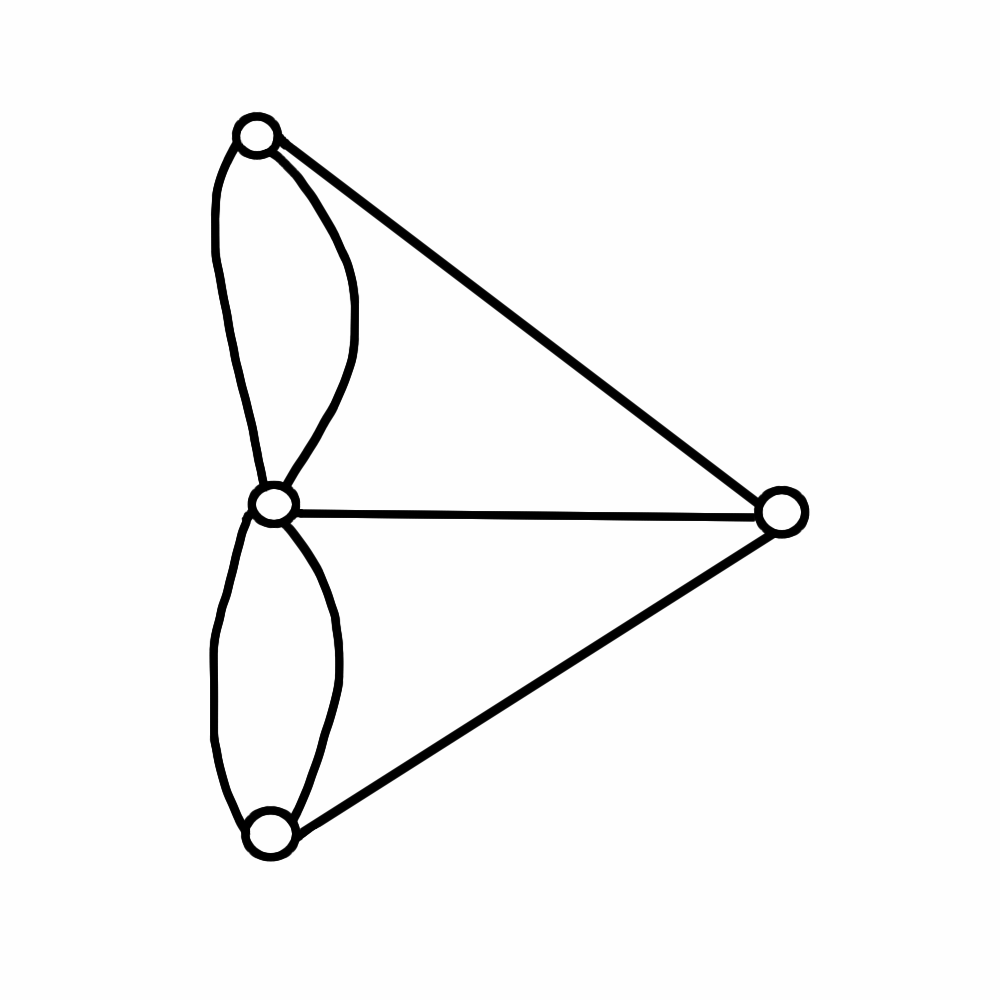
\includegraphics[width=.3\textwidth]{images/konigsberg-graph.png}
\caption{The K\"{o}nigsberg Bridges graph}
\label{figure:konigsberg-graph}
\end{figure}

How about for another graph?  What would we need to be true for a graph for 
there to be an Eulerian cycle on that graph?

Well, an Eulerian cycle has to be a cycle, first of all. Imagine walking along this cycle. At each vertex, 
the cycle has to enter and leave the same number of times. But to be an \emph{Eulerian} cycle, each 
edge has to be used exactly once. So, at each vertex there must be an even number of edges. That
means that each vertex must have even degree.

\begin{theorem}\label{thm:necessary} 
If a connected graph has an Eulerian cycle, then all of its vertices have even degree.
\end{theorem}

This is a useful thing to know. Already it helps us see that the K\"{o}nigsberg bridges problem
doesn't have a solution: \emph{all} of its vertices have odd degree. The people of K\"{o}nigsberg
didn't even have a chance.

\begin{exercise}
Use Theorem \ref{thm:necessary} to decide if the graphs $K_{3,3}$, $K_4$, and $K_6$ have an Eulerian cycle.
\end{exercise}

\begin{exercise}
Use Theorem \ref{thm:necessary} to settle the Five Rooms Puzzle.
\end{exercise}

\begin{exercise}\label{exercise:try}
Use Theorem \ref{thm:necessary} to design two interesting graphs that don't have Eulerian cycles.
Can you make it ``not obvious?''
\end{exercise}

The kind of thing in Theorem \ref{thm:necessary} is called a \emph{necessary} condition. This is because if
a graph is going to be Eulerian, it \textit{has} to satisfy this condition, too. It is necessary.

\subsection*{A Sufficient Condition}

Now, what can we say if a graph has the property that all of its vertices have even degree? It is necessary for the
graph to be Eulerian. Is it also \emph{sufficient}? That is, is the condition strong enough to not only rule out graphs
which are not Eulerian, but also to guarantee that a graph is Eulerian?

It turns out to be true. The necessary condition is also sufficient. We can improve our theorem to this one:

\begin{theorem}[Leonhard Euler, 1736] \label{thm:euler}
A connected graph has an Eulerian cycle if, and only when the degree of each of its vertices is even. 
That is, the two statements below are equivalent:
\begin{compactitem}
\item The graph $G$ is Eulerian.
\item The for every vertex $v$ of the graph $G$, the degree of $v$ is even.
\end{compactitem}
\end{theorem}

This result is widely credited with being the first result from graph theory. 

\begin{exercise}
Use Theorem \ref{thm:euler} to decide if the graphs $K_3$ and $K_5$ are Eulerian or not.
In general, for which values of $n$ is the graph $K_n$ an Eulerian graph?
\end{exercise}

Theorem \ref{thm:euler} is pretty amazing. Using it we can exactly answer the question of "is this graph
Eulerian," not by looking for paths, but by just counting edges at each vertex.

\subsection*{Algorithms, and a Proof of Euler's Theorem}

The best kind of solution to the (general) K\"{o}nigsberg bridge problem would be a sure-fire method for
finding an Eulerian cycle. What would that entail? It would be nice if we could find a simple set of instructions,
a recipe, for creating the Eulerian cycle. Those instructions should be really simple to follow, too, and we should
be sure that they would always work.

Such a process is called an \emph{algorithm}.  There are algorithms everywhere in your life, whether you realize it
or not. At some point you learned how to do the \emph{long division} algorithm. If you are lucky, maybe you 
learned to do \emph{Russian peasant multiplication} at some point.

Above, we saw an argument for why the condition on vertices is necessary. Now it is time to see an argument 
(a proof!) for why the condition on vertices is sufficient. The proof consists of an algorithm for for actually 
constructing the Eulerian cycle.

As you read this proof, please work through it for the example of the graph $G=K_5$.

\begin{proof}[Proof of Sufficiency]
Suppose that $G$ is a connected graph which has each of its vertices of even degree.

Label the vertices with counting numbers in any way you desire, but be sure to use an unbroken string of them:
\[
1, 2, 3, \ldots, V-1, V,
\]
where $V$ is the total number of vertices.

\begin{enumerate}
\item Start at the vertex labeled $1$. 
\item Follow an unused edge which joints $1$ to the smallest numbered vertex available. Mark this edge.
\item At this new vertex, follow whichever available unused edge leads to the smallest numbered vertex. Mark
the edge as you cross it.
\item Continue until you come back to vertex $1$.
\item If there are more edges attached to vertex $1$ which have not been used, repeat the process above
using only edges you have not previously marked. 
\item Put these cycles together by attaching them at the vertex $1$.
\item When all of the edges attached to vertex $1$ have been used. Go to the smallest numbered vertex which
has unused edges and do the process above for this vertex.
\item At some point, the process will stop, because each step involves decreasing the number of unused edges,
so you eventually run out. When this happens, you will have decomposed the graph into some number of cycles.
Because the graph is connected, each cycle must share a vertex with at least one other cycle. Choose such points
and splice the cycles together.
\end{enumerate}
\end{proof}

\begin{exercise}
Follow the steps of the proof to try to find Eulerian cycles in the graphs you made in Exercise \ref{exercise:try}.
Where does the process break?
\end{exercise}

\begin{exercise}
Why is it important that the graph have vertices of even degree? How might the algorithm break if you have 
a vertex of odd degree?
\end{exercise}

\begin{exercise}
Design a connected graph with at least seven vertices and a largish number of edges. Make sure that each
vertex has even degree. Apply the algorithm to your graph to find an Eulerian cycle.
\end{exercise}

\subsection*{A New Challenge}

Here is a variant of the K\"{o}nigsberg bridges puzzle: Suppose that you do not require your path to be a cycle.
That is, we don't necessarily want to start and end at the same place. But we do want to traverse each edge
exactly once. Can such a path be constructed?

In general, suppose $G$ is a connected graph. What must be true about the graph in order to find a path 
in the graph which uses each edge exactly once? Find a necessary condition.

Is that condition sufficient, too? How much of the work and ideas above can be reused?


%\begin{thebibliography}{9}
%\end{thebibliography}

\end{document}
%sagemathcloud={"zoom_width":100}










